\documentclass{article}
\usepackage[x11names, svgnames, rgb]{xcolor}
\usepackage[utf8]{inputenc}
\usepackage{tikz}
\usetikzlibrary{snakes,arrows,shapes}
\usepackage{amsmath}

\definecolor{lightcoral}{RGB}{240,128,128}
\definecolor{lightgreen}{RGB}{144,238,144}
%
%

%

%

\begin{document}
\pagestyle{empty}
%
%
%

\enlargethispage{100cm}
% Start of code
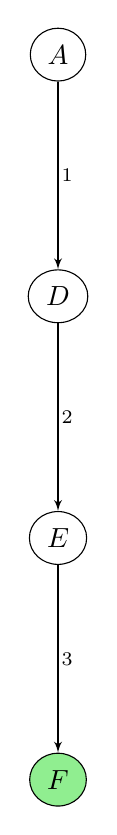
\begin{tikzpicture}[>=latex',line join=bevel,]
%%
\node (A) at (27.0bp,279.0bp) [draw,ellipse] {$A$};
  \node (D) at (27.0bp,192.0bp) [draw,ellipse] {$D$};
  \node (E) at (27.0bp,105.0bp) [draw,ellipse] {$E$};
  \node (F) at (27.0bp,18.0bp) [draw,fill=lightgreen,ellipse] {$F$};
  \draw [->] (A) ..controls (27.0bp,249.19bp) and (27.0bp,233.56bp)  .. (D);
  \definecolor{strokecol}{rgb}{0.0,0.0,0.0};
  \pgfsetstrokecolor{strokecol}
  \draw (30.5bp,235.5bp) node {$_1$};
  \draw [->] (D) ..controls (27.0bp,162.19bp) and (27.0bp,146.56bp)  .. (E);
  \draw (30.5bp,148.5bp) node {$_2$};
  \draw [->] (E) ..controls (27.0bp,75.192bp) and (27.0bp,59.561bp)  .. (F);
  \draw (30.5bp,61.5bp) node {$_3$};
%
\end{tikzpicture}
% End of code

%
\end{document}
%



